\documentclass[11pt,a4paper]{article}
\usepackage{a4wide,url,graphicx}
\usepackage[utf8]{inputenc}
\usepackage[russian]{babel}
\usepackage{tikz}
\usetikzlibrary{shapes.misc}
\usetikzlibrary{arrows.meta}

\parskip3pt
\parindent0pt

\title{Different Versions of the Laws of\\ Technical Evolution within TRIZ}

\author{Compiled by Hans-Gert Gräbe, Leipzig}

\date{Version of 07 December 2019}

\begin{document}
\maketitle

\section*{The version as presented in the improved TDS material}

The following diagram was compiled using the \texttt{tikz} \LaTeX-package from
the corresponding (improved) diagram in the Exercises of the TRIZ Summit
Cup\footnote{\url{https://triz-summit.ru/contest/cup-tds-2019-2020/contest-2019-2020/}}.

\begin{center}
\newcommand{\law}[2]{\parbox{#1cm}{\small\centering #2}}
\tikz[>={Triangle[length=3pt 9, width=3pt 3]}] {
  
\node[draw] at (5,7) [rectangle]
(A1) {\law{3}{Закон повышения идеальности}};

\node[draw] at (0,6) [rectangle]
(A2) {\law{4}{Закон повышения полноты частей системы (Закон полноты выполнения принципа действия)}};

\node[draw] at (0,2) [rectangle]
(A3) {\law{4}{Закон повышения согласованности частей системы}};

\node[draw] at (0,4) [rectangle]
(A4) {\law{4}{Закон проводимости: энергии, потоков и др.}};

\node[draw] at (5,5) [rectangle]
(A5) {\law{3}{Закон неравномерного развития частей системы}};

\node[draw] at (10,0) [rectangle]
(A6) {\law{4}{Тенденция развития ТС по S-образной кривой}};

\node[draw] at (0,0) [rectangle]
(A7) {\law{4}{Тенденция вытеснения человека из ТС}};

\node[draw] at (10,4) [rectangle]
(A8) {\law{4}{Закон повышения управляемости / вепольности}};

\node[draw] at (5,1) [rectangle]
(A9) {\law{3}{Закон повышения динамичности}};

\node[draw] at (5,3) [rectangle]
(A10) {\law{3}{Закон перехода в надсистему}};

\node[draw] at (10,6) [rectangle]
(A11) {\law{4}{Закон перехода с макроуровня на микроуровень}};

\node[draw] at (10,2) [rectangle]
(A12) {\law{4}{Тенденция развития за счет свертывания или развертывания ТС}};

\draw[->] (A1) -- (2.8,7) |- (A2) ;
\draw[->] (2.8,7) |- (A3);
\draw[->] (2.8,7) |- (A4);
\draw[->] (2.8,7) |- (A5);
\draw[->] (2.8,7) |- (A7);
\draw[->] (2.8,7) |- (A9);
\draw[->] (2.8,7) |- (A10);
\draw[->] (A2) -- (-2.7,6) |- (A7);
\draw[->] (A5) -- (7.2,5) |- (A9);
\draw[->] (7.2,5) |- (A10);
\draw[->] (7.2,5) |- (A6);
\draw[->] (A1) -- (7.5,7) |- (A8) ;
\draw[->] (7.5,7) |- (A11) ;
\draw[->] (7.5,7) |- (A12) ;
\draw[->] (A8) -- (12.5,4) |- (A12) ;
}
\end{center}

\section*{The Laws as given in the irst version of the TDS material}

\begin{center}
  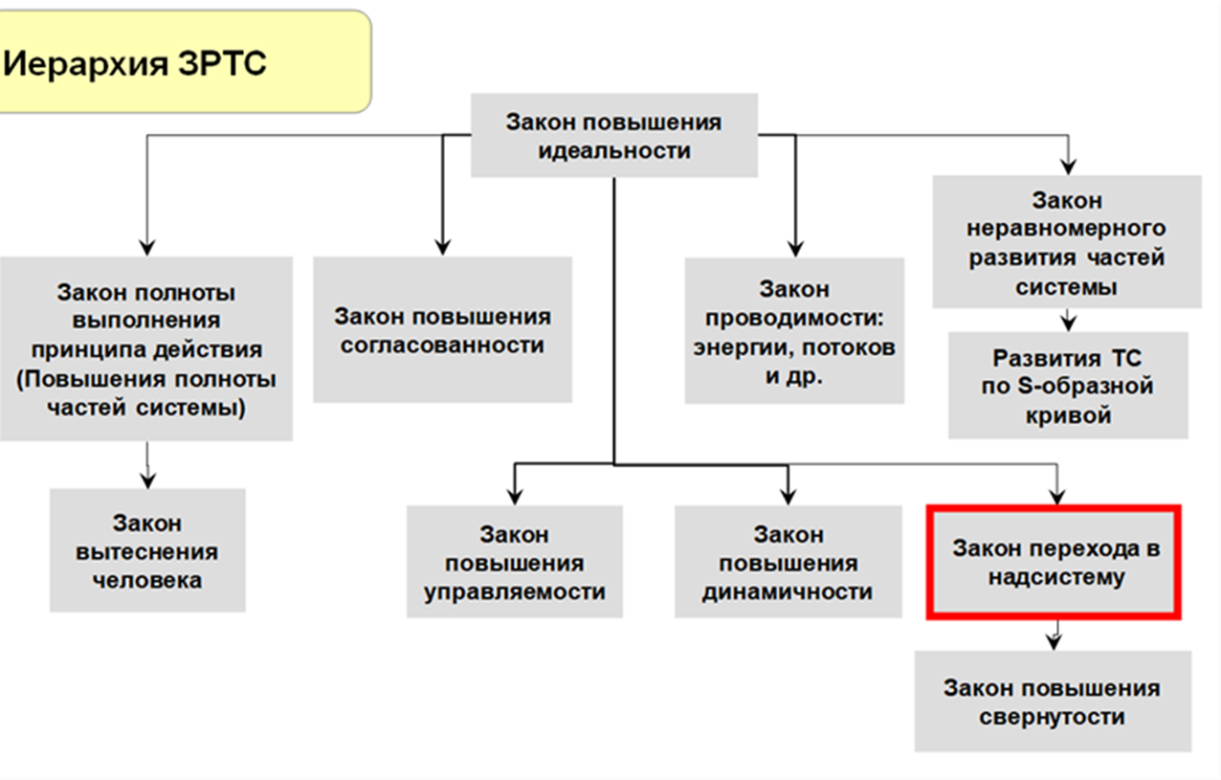
\includegraphics[width=.9\textwidth]{oE4yUs.png}
\end{center}

\section*{Laws as explained in (Koltze/Souchkov, ch. 4.8)}

(Koltze/Souchkov) distinguish between laws at the one side and evolutionary
lines and trends of the development of technical systems on the other side.

Laws of evolution of technical systems
\begin{enumerate}\itemsep0pt
\item Law of the completeness of the system
\item Law of completeness of the supersystem
\item Law of increasing ideality
\item Law of uneven development of system parts
\item Law of increasing substance-field interactions
\end{enumerate}

Evolution lines and trends of technical systems
\begin{enumerate}\itemsep0pt
\item Dynamization
\item Coordination and Evolution of Rhythm
\item Coordination of shape and form
\item Evolution of geometry
\item Increasing Energy Conductivity
\item Transition to the micro level
\item Increasing controllability
\item Increasing automation
\item Transition to the upper system
\item Coincidence
\end{enumerate}

\subsection*{German Original}

Gesetze der Evolution technischer Systeme
\begin{enumerate}\itemsep0pt
\item Gesetz der Vollständigkeit des Systems
\item Gesetz der Vollständigkeit des Obersystems
\item Gesetz der Erhöhung der Idealität
\item Gesetz der ungleichen Entwicklung von Systemteilen
\item Gesetz der Erhöhung von Stoff-Feld-Interaktionen
\end{enumerate}

Evolutionslinien und -trends technischer Systeme
\begin{enumerate}\itemsep0pt
\item Dynamisierung
\item Koordination und Evolution der Rhythmik
\item Gestalt- und Formkoordination
\item Evolution der Geometrie
\item Erhöhung des Energie-Leitvermögens
\item Übergang auf die Mikroebene
\item Zunehmende Steuerbarkeit
\item Erhöhung der Automation
\item Übergang zum Obersystem
\item Zusammenfall
\end{enumerate}



\end{document}
